
\begin{figure}
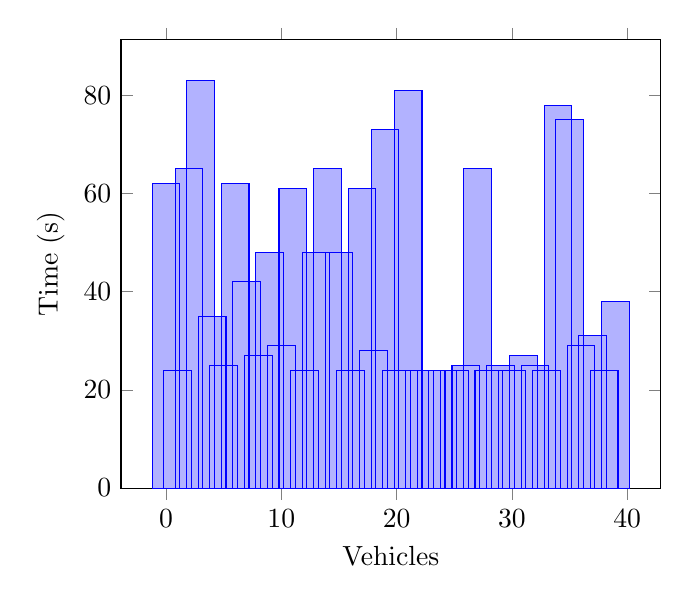
\begin{tikzpicture}
\begin{axis}[
legend style={anchor=west},
xlabel=Vehicles,
ylabel=Time (s),
ymin=0,
ybar,
]
\addplot coordinates {
(0, 62)
(1, 24)
(2, 65)
(3, 83)
(4, 35)
(5, 25)
(6, 62)
(7, 42)
(8, 27)
(9, 48)
(10, 29)
(11, 61)
(12, 24)
(13, 48)
(14, 65)
(15, 48)
(16, 24)
(17, 61)
(18, 28)
(19, 73)
(20, 24)
(21, 81)
(22, 24)
(23, 24)
(24, 24)
(25, 24)
(26, 25)
(27, 65)
(28, 24)
(29, 25)
(30, 24)
(31, 27)
(32, 25)
(33, 24)
(34, 78)
(35, 75)
(36, 29)
(37, 31)
(38, 24)
(39, 38)
};

\end{axis}
\end{tikzpicture}
\label{tik:0:3_V, 3_V.-60, 2_V}
\caption{0 percent diving with GSC on route $3_V, 3_V.-60, 2_V$}
\end{figure}
